\documentclass[a4paper,12pt]{article}
\usepackage{../../../mypackages}
\usepackage{../../../macros}


\usepackage{pgfplots}
    \pgfplotsset{
    compat=1.11,
  }

\setlength{\parindent}{0pt}


\begin{document}

\title{Corrigé exercices à faire pour le 13 Septembre}
\author{N. Bancel}

\maketitle

\section*{Exercice N°13 page 164}

\begin{tcolorbox}[colback=yellow!10!white, colframe=yellow!50!black, title=Méthode pour vérifier l'appartenance d'un point à une courbe]
  Pour déterminer si un point \( P(a, b) \) appartient à la courbe représentative d'une fonction \( g(x) \), il suffit de vérifier si l'ordonnée \( b \) du point correspond à l'image de l'abscisse \( a \) par la fonction \( g(x) \). Cela revient à calculer \( g(a) \) et comparer cette valeur avec \( b \). Si \( g(a) = b \), alors le point \( P(a, b) \) appartient à la courbe. Sinon, le point n'appartient pas à la courbe.
  \end{tcolorbox}

\begin{figure}[H]
    \centering
    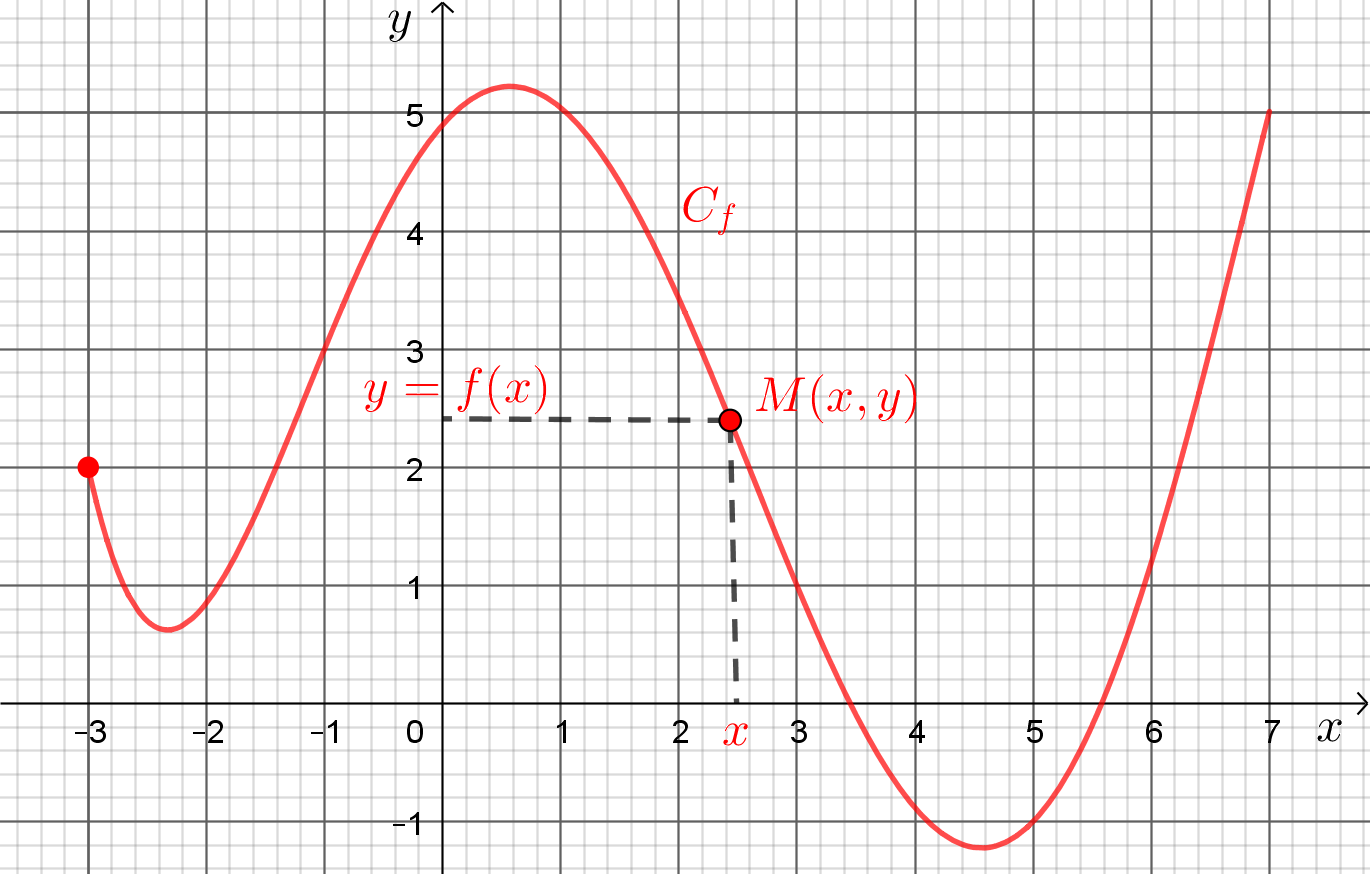
\includegraphics[width=0.5\linewidth]{exos_1.png}
    \caption{\label{} Appartenance d'un point à une courbe}
  \end{figure}
  
  La fonction étudiée est \( g(x) = x^2 - 3x + 2 \). Nous allons calculer \( g(x) \) pour chaque abscisse des points et comparer avec leur ordonnée.
  
  \textbf{Point \( A(0, 2) \)} \par 
  Calculons \( g(0) \) :
  \[
  g(0) = 0^2 - 3(0) + 2 = 2
  \]
  L'ordonnée du point \( A \) est \( 2 \), et \( g(0) = 2 \). Donc, le point \( A(0, 2) \) appartient à la courbe.
  
  \textbf{2. Point \( B(-1, 6) \)} \par 
  Calculons \( g(-1) \) :
  \[
  g(-1) = (-1)^2 - 3(-1) + 2 = 1 + 3 + 2 = 6
  \]
  L'ordonnée du point \( B \) est \( 6 \), et \( g(-1) = 6 \). Donc, le point \( B(-1, 6) \) appartient à la courbe.
  
  \textbf{3. Point \( C(2, 0) \)} \par 
  Calculons \( g(2) \) :
  \[
  g(2) = 2^2 - 3(2) + 2 = 4 - 6 + 2 = 0
  \]
  L'ordonnée du point \( C \) est \( 0 \), et \( g(2) = 0 \). Donc, le point \( C(2, 0) \) appartient à la courbe.
  
  \textbf{4. Point \( D(1, 0) \)} \par

  Calculons \( g(1) \) :
  \[
  g(1) = 1^2 - 3(1) + 2 = 1 - 3 + 2 = 0
  \]
  L'ordonnée du point \( D \) est \( 0 \), et \( g(1) = 0 \). Donc, le point \( D(1, 0) \) appartient à la courbe.
  
  \section*{Exercice N°39 page 164}


  \begin{tcolorbox}[colback=yellow!10!white, colframe=yellow!50!black, title=Méthode pour vérifier une forme factorisée]
    Pour montrer qu'une expression sous forme factorisée est équivalente à une forme développée, il suffit de développer la forme factorisée en appliquant les règles de distributivité. Ensuite, on compare les termes obtenus avec ceux de l'expression initiale. Si les termes correspondent, la factorisation est correcte.
    \end{tcolorbox}
    
    Nous cherchons à résoudre l'équation suivante :
    \[
    2x^2 - 14x = -24
    \]
    Cette équation peut être réécrite sous la forme :
    \[
    2x^2 - 14x + 24 = 0
    \]
    
    \subsection*{1. Démonstration de la forme factorisée}
    Nous devons montrer que :
    \[
    2x^2 - 14x + 24 = 2(x - 3)(x - 4)
    \]
    
    Pour cela, développons la forme factorisée \( 2(x - 3)(x - 4) \) :
    \[
    2(x - 3)(x - 4) = 2 \times [(x - 3)(x - 4)]
    \]
    Développons \( (x - 3)(x - 4) \) :
    \[
    (x - 3)(x - 4) = x(x - 4) - 3(x - 4) = x^2 - 4x - 3x + 12 = x^2 - 7x + 12
    \]
    Ensuite, multiplions le résultat par 2 :
    \[
    2(x^2 - 7x + 12) = 2x^2 - 14x + 24
    \]
    
    Nous obtenons bien l'expression initiale \( 2x^2 - 14x + 24 \), ce qui montre que la factorisation est correcte :
    \[
    2x^2 - 14x + 24 = 2(x - 3)(x - 4)
    \]
    
    \subsection*{2. Résolution de l'équation \( 2x^2 - 14x = -24 \)}
    L'équation à résoudre est :
    \[
    2x^2 - 14x + 24 = 0
    \]
    
    Grâce à la factorisation, nous avons :
    \[
    2(x - 3)(x - 4) = 0
    \]
    
    Pour que le produit soit nul, il faut que l'un des deux facteurs soit nul :
    \[
    x - 3 = 0 \quad \text{ou} \quad x - 4 = 0
    \]
    
    Les solutions sont donc :
    \[
    x = 3 \quad \text{ou} \quad x = 4
    \]
    
    \textbf{Conclusion :} Les solutions de l'équation \( 2x^2 - 14x = -24 \) sont \( x = 3 \) et \( x = 4 \).
  

    \subsection*{3. [Optionnel mais assez intéressant] Vérification des solutions}

    Il est intéressant de vérifier que les solutions \( x = 3 \) et \( x = 4 \) sont bien des solutions de l'équation initiale \( 2x^2 - 14x = -24 \). Nous allons donc substituer ces valeurs dans la forme développée.

    Pour \( x = 3 \) :
\[
2x^2 - 14x + 24 = 2(3)^2 - 14(3) + 24 = 2 \times 9 - 42 + 24 = 18 - 42 + 24 = 0
\]
L'égalité est vérifiée.

Pour \( x = 4 \) :
\[
2x^2 - 14x + 24 = 2(4)^2 - 14(4) + 24 = 2 \times 16 - 56 + 24 = 32 - 56 + 24 = 0
\]
L'égalité est également vérifiée.

\textbf{Conclusion :} Les solutions de l'équation \( 2x^2 - 14x = -24 \) sont \( x = 3 \) et \( x = 4 \), et elles satisfont bien l'équation initiale.

    \section*{Exercice N°42 page 170}
    
    \begin{tcolorbox}[colback=yellow!10!white, colframe=yellow!50!black, title=Attention aux signes]
    Lorsqu'on factorise ou développe des expressions algébriques, il est essentiel de faire très attention aux signes (positifs et négatifs) afin d'éviter les erreurs d'étourderie. En particulier, dans cet exercice, chaque terme négatif doit être manipulé avec soin lors de la factorisation et du développement pour obtenir des résultats corrects.
    \end{tcolorbox}
    
    Nous cherchons à résoudre l'équation suivante :
    \[
    -x^2 - 3x - 2 = 0
    \]
    
    \subsection*{1. Démonstration de la forme factorisée}
    Nous devons montrer que :
    \[
    -x^2 - 3x - 2 = -(x + 2)(x + 1)
    \]
    
    Pour cela, développons \( -(x + 2)(x + 1) \) :
    \[
    -(x + 2)(x + 1) = -[(x + 2)(x + 1)]
    \]
    Développons \( (x + 2)(x + 1) \) :
    \[
    (x + 2)(x + 1) = x(x + 1) + 2(x + 1) = x^2 + x + 2x + 2 = x^2 + 3x + 2
    \]
    
    Ensuite, multiplions tout par \( -1 \) :
    \[
    -(x^2 + 3x + 2) = -x^2 - 3x - 2
    \]
    
    Nous obtenons bien l'expression initiale \( -x^2 - 3x - 2 \), ce qui montre que la factorisation est correcte :
    \[
    -x^2 - 3x - 2 = -(x + 2)(x + 1)
    \]
    
    \subsection*{2. Résolution de l'équation \( -x^2 - 3x - 2 = 0 \)}
    L'équation à résoudre est :
    \[
    -x^2 - 3x - 2 = 0
    \]
    
    Grâce à la factorisation, nous avons :
    \[
    -(x + 2)(x + 1) = 0
    \]
    
    Pour que le produit soit nul, il faut que l'un des deux facteurs soit nul :
    \[
    x + 2 = 0 \quad \text{ou} \quad x + 1 = 0
    \]
    
    Les solutions sont donc :
    \[
    x = -2 \quad \text{ou} \quad x = -1
    \]
    
    \textbf{Conclusion :} Les solutions de l'équation \( -x^2 - 3x - 2 = 0 \) sont \( x = -2 \) et \( x = -1 \).

    \subsection*{3. [Optionnel mais assez intéressant] Vérification des solutions}

    Il est intéressant de vérifier que les solutions \( x = -2 \) et \( x = -1 \) sont bien des solutions de l'équation initiale \( -x^2 - 3x - 2 = 0 \). Nous allons donc substituer ces valeurs dans la forme développée.

Pour \( x = -2 \) :
\[
-x^2 - 3x - 2 = -(-2)^2 - 3(-2) - 2 = -4 + 6 - 2 = 0
\]
L'égalité est vérifiée.

Pour \( x = -1 \) :
\[
-x^2 - 3x - 2 = -(-1)^2 - 3(-1) - 2 = -1 + 3 - 2 = 0
\]
L'égalité est également vérifiée.

\vspace{1em}

\textbf{Conclusion :} Les solutions \( x = -2 \) et \( x = -1 \) sont bien correctes pour l'équation \( -x^2 - 3x - 2 = 0 \).

\section*{Exercice N°47 page 171}

\begin{tcolorbox}[colback=yellow!10!white, colframe=yellow!50!black, title=Méthode pour trouver la seconde solution]
  Lorsque l'on connaît une solution d'une équation quadratique du type \( ax^2 + bx + c = 0 \), on peut utiliser la méthode de la factorisation. En sachant qu'une des solutions est donnée, on peut écrire l'équation sous forme factorisée, puis retrouver la seconde solution en résolvant l'autre facteur.
\end{tcolorbox}

\subsection*{\(x^2 - 3x + 2 = 0\) sachant qu'une solution est 1}

\textbf{Étape 1 : Utiliser la forme factorisée}
Puisque \( x = 1 \) est une solution de l'équation, nous pouvons factoriser le polynôme sous la forme :
\[
x^2 - 3x + 2 = (x - 1)(x - r) = 0
\]
où \( r \) est la seconde solution que nous devons déterminer.

\textbf{Étape 2 : Développer la forme factorisée}
Développons l'expression \( (x - 1)(x - r) \) pour l'égaliser à la forme \( x^2 - 3x + 2 \) :
\[
(x - 1)(x - r) = x(x - r) - 1(x - r) = x^2 - rx - x + r = x^2 - (r + 1)x + r
\]

\textbf{Étape 3 : Comparaison des coefficients}
En comparant les coefficients de l'expression développée avec ceux de l'équation initiale \( x^2 - 3x + 2 \), nous obtenons :
\[
-(r + 1) = -3 \quad \text{et} \quad r = 2
\]

\textbf{Étape 4 : Résolution}

Nous trouvons que \( r = 2 \).

Le polynôme peut donc s'écrire sous la forme factorisée \((x - 1)(x - 2)\)

\textbf{Étape 5 : Conclusion}
La seconde solution de l'équation \( x^2 - 3x + 2 = 0 \) est donc :
\[
x = 2
\]

\textbf{Vérification des solutions}
Nous pouvons vérifier que les solutions \( x = 1 \) et \( x = 2 \) sont correctes en substituant ces valeurs dans l'équation initiale.

Pour \( x = 1 \) :
\[
x^2 - 3x + 2 = 1^2 - 3 \times 1 + 2 = 1 - 3 + 2 = 0
\]
L'égalité est vérifiée.

Pour \( x = 2 \) :
\[
x^2 - 3x + 2 = 2^2 - 3 \times 2 + 2 = 4 - 6 + 2 = 0
\]
L'égalité est également vérifiée.

\textbf{Conclusion :} Les solutions de l'équation \( x^2 - 3x + 2 = 0 \) sont \( x = 1 \) et \( x = 2 \).

\subsection*{\(x^2 + 7x + 12 = 0\) sachant qu'une solution est -4}

Sachant que l'une des solutions est \( x = -4 \), on factorise ainsi :
\[
x^2 + 7x + 12 = (x + 4)(x - r)
\]
En développant :
\[
(x + 4)(x - r) = x^2 + (4 - r)x - 4r
\]
En comparant avec \( x^2 + 7x + 12 \), on a \( 4 - r = 7 \) et \( -4r = 12 \), donc \( r = -3 \).

La seconde solution est donc \( x = -3 \).

\textbf{Vérification} : 
Pour \( x = -4 \), \( (-4)^2 + 7(-4) + 12 = 0 \).

Pour \( x = -3 \), \( (-3)^2 + 7(-3) + 12 = 0 \).

Les solutions sont correctes.

\subsection*{\(2x^2 + 10x + 12 = 0\) sachant qu'une solution est -2}

L'équation est :
\[
2x^2 + 10x + 12 = 0
\]
Sachant que \( x = -2 \) est une solution, on divise par 2 :
\[
x^2 + 5x + 6 = 0
\]
On factorise :
\[
x^2 + 5x + 6 = (x + 2)(x + r)
\]
En développant, on obtient \( (x + 2)(x + r) = x^2 + (2 + r)x + 2r \), donc \( 2 + r = 5 \) et \( 2r = 6 \). D'où \( r = 3 \).

La seconde solution est donc \( x = -3 \).

\textbf{Vérification} : 
Pour \( x = -2 \), \( 2(-2)^2 + 10(-2) + 12 = 0 \).

Pour \( x = -3 \), \( 2(-3)^2 + 10(-3) + 12 = 0 \).

Les solutions sont correctes.

\subsection*{\(3x^2 + 24x + 36 = 0\) sachant qu'une solution est -6}

L'équation est :
\[
3x^2 + 24x + 36 = 0
\]
Sachant que \( x = -6 \) est une solution, on divise par 3 :
\[
x^2 + 8x + 12 = 0
\]
On factorise :
\[
x^2 + 8x + 12 = (x + 6)(x + r)
\]
En développant, on a \( (x + 6)(x + r) = x^2 + (6 + r)x + 6r \), donc \( 6 + r = 8 \) et \( 6r = 12 \). D'où \( r = 2 \).

La seconde solution est donc \( x = -2 \).

\textbf{Vérification} : 
Pour \( x = -6 \), \( 3(-6)^2 + 24(-6) + 36 = 0 \).

Pour \( x = -2 \), \( 3(-2)^2 + 24(-2) + 36 = 0 \).

Les solutions sont correctes.

  \end{document}
